\documentclass[a4paper,12pt]{article}
\usepackage[utf8]{inputenc}
\usepackage[T1]{fontenc}
\usepackage[spanish, es-tabla]{babel}
\usepackage{mathrsfs}
\usepackage{amssymb,amsmath}
\usepackage{enumerate}
% \usepackage{enumitem}  % It's better than enumerate
% \usepackage{capt-of}
% \usepackage{multicol}
\usepackage{multirow}
\usepackage{caption}
\usepackage{graphicx}
% \usepackage{ifthen}
\usepackage{xcolor}
% \usepackage{tabularx}
% \usepackage{hyperref}
\usepackage{url}

\usepackage[locale=FR, per-mode=fraction, separate-uncertainty=true]{siunitx}
\usepackage{physics}
% \usepackage{algorithm}

\usepackage[style=numeric, sorting=none]{biblatex}
\addbibresource{refs.bib}


\usepackage{pgfplots}
\usepackage{tikz}
% \usepackage{circuitikz}  % includes tikz
% \usepackage{tikz-3dplot}
\usepackage{gnuplottex}

\usetikzlibrary{decorations.pathreplacing,shapes,patterns,calc}
\usetikzlibrary{babel}
\usetikzlibrary{decorations}
\usetikzlibrary{decorations.pathmorphing}
\usetikzlibrary{shapes.geometric}
\usetikzlibrary{arrows}
\usetikzlibrary{arrows.meta}   %edg
\usetikzlibrary{calc}
\usetikzlibrary{patterns}
\pgfplotsset{compat=newest}  %sin esto, no hace bien el gráfico


\usepackage[a4paper,vmargin={15mm,20mm},hmargin={20mm,15mm}, includefoot, bottom=3.5cm]{geometry}
\usepackage{fancybox}
% \usepackage{lastpage}
\usepackage{fancyhdr}
\setlength{\headheight}{60pt}
\pagestyle{fancy}
\fancyhead{}
\rhead{2\textsuperscript{do} 31 - 2026}
\lhead{\input{../logoFRA.tex}}
\chead{Laboratorio de Física II}
% \rfoot{\thepage\ / \pageref{LastPage}}
% \cfoot{}
% \lfoot{\textit{hola}}
% \renewcommand{\footrulewidth}{0.4pt}


\newcounter{preguntas}

\begin{document}
\thispagestyle{fancy}

\vspace*{10pt}

\begin{center}
    % \huge FÍSICA II\\[10pt]
    \LARGE Trabajo práctico nro. 2: \\[10pt]
    \LARGE Ley de Biot-Savart
\end{center}
    
\vspace{20pt}

\section*{Objetivos}

\begin{itemize}
\item Comprobar experimentalmente que la circulación de una corriente eléctrica genera un campo magnético.
\item Medir la intensidad del campo magnético terrestre en el laboratorio.
\end{itemize}

\section*{Introducción}

En esta experiencia se determinará la magnitud del campo magnético de la Tierra en el sitio geográfico donde está ubicado el laboratorio donde se realizn las mediciones. El campo magnético terrestre se asemeja al campo generado por una barra magnetizada, y el polo sur magnético se ubica cerca del polo norte geográfico \cite[pp.~883-885]{young_freedman_2013}. Siendo que la aguja de una brújula es un pequeño imán, ésta siente un torque magnético que tiende a alinearla con el campo magnético externo \cite[p.~903]{young_freedman_2013}. Debido a que polos opuestos se atraen, el polo norte de la aguja apunta hacia el polo sur magnético de la Tierra.\par\medskip

La determinación de un campo magnético desconocido (en este caso, el campo terrestre) se puede realizar creando un campo adicional conocido, y para ello en esta experiencia se utiliza una espira circular. El campo que se genera en el centro de una espira circular de radio $a$, cuando circula una corriente $i$, es perpendicular a la espira y su módulo es \cite[pp.~933-934]{young_freedman_2013}:
\begin{equation}\label{Bespira}
B = \frac{\mu_o i}{2a}\, ,
\end{equation}
donde $\mu_0$ es la permeabilidad del vacío, y su valor experimental recomendado es $\SI{1.25663706127(20)E-6}{NA^{-2}}$ \cite{nist_mu0_2022}.\par\medskip

En particular, en el centro de la espira, el campo neto será la suma del campo generado por la espira, $\va*{B}_{\text{E}}$, y el campo magnético de la Tierra, $\va*{B}_{\text{T}}$:
\begin{equation}\label{suma}
\va*{B}_{\text{R}} = \va*{B}_{\text{E}} + \va*{B}_{\text{T}}\, .
\end{equation}

Si en el centro de la espira se ubica una espira, esta rotará para alinearse al campo resultante, y midiendo las deflexiones de la aguja se podrá determinar el valor del campo magnético terrestre, como se explica en la siguiente sección.\par\medskip

Es necesario agregar que al momento de sumar los vectores, se deberá considerar que el campo magnético terrestre generalmente no es paralelo a la superficie de la Tierra. Para obtener la inclinación magnética se puede utilizar el sitio para la estimación del campo magnético terrestre de ``National Oceanic and Atmospheric Administration (NOAA)'' \cite{noaa_magcalc_2026}. En el caso de Villa Domínico, Avellaneda, Provincia de Buenos Aires, Argentina, con latitud $-34.691667$ y longitud $-58.333333$, la inclinación (vertical) es $\SI{41.3148}{\degree}$ hacia arriba.


\section*{Materiales}
\begin{itemize}
    \item Brújula
    \item Espira de cobre
    \item Fuente de tensión (6V C.C.)
    \item Amperímetro
    \item Resistencia variable
\end{itemize}


\section*{Desarrollo de la experiencia}

Se conecta una espira circular en serie con una resistencia variable, una fuente de voltaje, y un amperímetro, como se muestra en el esquema de la figura \ref{circuito}.
\begin{figure}[!ht]
\begin{center}
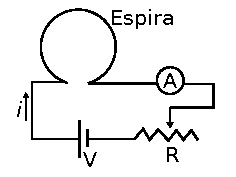
\includegraphics[scale=1.2]{TP_biot_circuito.pdf}
\caption{Circuito que alimenta la espira.}\label{circuito}
\end{center}
\end{figure}

Se ubica la brújula en el centro de la espira, de forma tal que la superficie de la espira sea tangente a la aguja cuando no circula corriente por el circuito. Debido a que la brújula esta diseñada de forma tal que la aguja pueda rotar en un plano horizontal, dicha aguja estará alineada con la proyección del campo magnético terrestre sobre el plano de rotación. Si definimos un sistema de referencia tal que en estas condiciones la aguja apunta hacia la dirección $+\vu{x}$, y el eje de simetría de la espira es paralelo al eje $+\vu{y}$, entonces el campo magnético terrestre tendrá componentes tanto en $\vu{x}$ como en $\vu{z}$:
\begin{equation}\label{inclinacion}
    \va*{B}_\text{T} = B_{\text{T},x}\,\vu{x} + B_{\text{T},z}\,\vu{z}\, .
\end{equation}

Cuando la corriente comience a circular, la espira producirá un campo magnético en su centro alineado con el eje $\vu{y}$:
\begin{equation}
    \va*{B}_\text{E} = B_{\text{E}}\,\vu{y}\, .
\end{equation}

Según la ecuación \ref{suma}, obtenemos lo siguiente para el campo resultante en el centro de la espira:
\begin{equation}
    \va*{B}_\text{R} = B_{\text{T},x}\,\vu{x} + B_{\text{E}}\,\vu{y} + B_{\text{T},z}\,\vu{z}\, .
\end{equation}

La aguja rotará para alinearse con la proyección sobre el plano $xy$ de este campo resultante, formando un ángulo $\theta$ respecto del eje $\vu{x}$. El ángulo del vector $\va*{B}_\text{R}$ respecto del eje $\vu{x}$ cumple con la siguiente ecuación:\\
\begin{equation}\label{theta}
\tan \theta = \frac{B_\text{E}}{B_{\text{T},x}}\, .
\end{equation}

Variando la resistencia $R$ del circuito, se hacen circular diferentes intensidades de corriente. Para cada una de ellas, se mide el ángulo que rota la aguja y se vuelcan los valores en una tabla.\par\medskip

Para cada una de las corrientes medidas, se debe calcular el valor del campo generado por la espira con la ecuación \ref{Bespira}. Graficar estos valores en función de las corrientes (un gráfico $B_\text{E}$ \textit{vs} $i$) y analizar si es el gráfico esperado para una espira circular.\par\medskip

Reordenando la ecuación \ref{theta} como $B_\text{E} = B_{\text{T},x}\tan \theta$, podemos ver que existe una relación lineal entre $B_\text{E}$ y $\tan \theta$, puesto que esperamos que el valor de $B_{\text{T},x}$ sea constante. Realizar un gráfico $B_\text{E}$ \textit{vs} $\tan \theta$ y analizar si se observa lo esperado.\par\medskip

A continuación, realizar un ajuste lineal a los valores del último gráfico. El valor de la pendiente será el valor de la proyección del campo terrestre sobre el plano $xy$, $B_{\text{T},x}$. Para obtener la magnitud del campo magnético terrestre, se deberá tener en cuenta el ángulo de inclinación vertical, $\phi$ (sobre el eje $\vu{z}$), de forma que a partir de la ecuación \ref{inclinacion}, el resultado es 
\begin{equation}\label{modulo}
    \left | \va*{B}_\text{T} \right | = \frac{B_{\text{T},x}}{\cos \phi}\, .
\end{equation}

\printbibliography 

\appendix

\section{Cálculo de los errores por propagación}

En este curso vamos a usar una versión simplificada del tratamiento estadístico correcto \cite{baird1991experimentacion}. Si consideramos una cantidad $y$ que se calcula a partir de las mediciones $x_1, x_2, \dots, x_N$ con una determinada función $f$ de varias variables:
\begin{equation}\label{eq:yfx}
    y = f(x_1,x_2,\dots,x_N)
\end{equation}
una forma de calcular el error de dicha cantidad es mediante la siguiente fórmula:
\begin{equation}\label{parciales}
    \varepsilon_y = \sum_i \left | \frac{\partial f}{\partial x_i} \right | \varepsilon_{x_i}
\end{equation}
donde $\varepsilon_{x_i}$ es la incerteza de la medición $x_i$.\par\medskip

En esta experiencia, la cantidad $\tan \theta$ es calculada a partir de las mediciones del ángulo que forma la aguja. Si la incerteza en la medición del ángulo es $\varepsilon_{\theta}$, utilizando la fórmula de la ecuación \ref{parciales}, el error en la tangente del ángulo resulta
\begin{equation}
    \varepsilon_{\tan \theta} = \sec^2(\theta) \varepsilon_{\theta}\, . 
\end{equation}

Debido a que el valor del campo generado por la espira debe ser calculado a partir de las diferentes mediciones de corriente, su error también puede ser calculado de la misma forma. Si la incerteza en el radio es $\varepsilon_a$ y en la corriente es $\varepsilon_i$, el error del campo generado por la espira que se obtiene mediante la ecuación \ref{parciales} es
\begin{equation}
    \varepsilon_{B_\text{E}} = \frac{\mu_0}{2a}\varepsilon_i + \frac{\mu_0 i}{2a^2}\varepsilon_{a}\, .
\end{equation}

\section{Calcular la incerteza de la pendiente en el ajuste lineal}

Cuando se utiliza un programa para realizar un ajuste lineal sobre un conjunto de puntos, se obtendrá el valor de la pendiente $m$, y el coeficiente de determinación $R^2$, que informa qué tan bien se adaptan los puntos experimentales a la recta que se obtuvo.\par\medskip

El valor de $R^2$ puede ser utilizado para calcular el error estándar (incerteza) de la pendiente $m$ utilizando la siguiente fórmula:

\begin{equation}\label{eq_corriente}
    \sigma = |m| \sqrt{\frac{\frac{1}{R^2}-1}{n-2}}\, ,
\end{equation}

donde $n$ es la cantidad de mediciones. En esta experiencia se está determinando el valor de un campo magnético mediante un ajuste lineal. Por lo tanto, el resultado final del ajuste lineal puede ser informado como
\begin{equation}
    (m \pm \sigma)\text{ T}\, .
\end{equation}

Recordar que en esta experiencia, la pendiente representa la componente $x$ del campo terrestre. Al calcular el módulo del campo terrestre con la ecuación \ref{modulo}, se debe propagar el error de la componente $x$ utilizando el método de derivadas parciales, de la misma forma que se utilizó para las demás cantidades.

\section{Cómo citar este documento:}
Si utiliza esta guía de laboratorio para sus informes o trabajos de investigación, puede citarla siguiendo el ejemplo a continuación:\par\medskip

E. Palazzo, \textit{Trabajo práctico nro. 2: Ley de Biot-Savart}. Universidad Tecnológica Nacional - Facultad Regional Avellaneda, Buenos Aires, Argentina, 2026. [En línea]. Disponible en: \url{https://raw.githubusercontent.com/frautn/F2/refs/heads/main/tpsLaboratorio/TP_BiotSavart/TP_BiotSavart_2026.pdf}

\end{document}
